\documentclass{article}
\usepackage{amsmath}
\usepackage{booktabs}
\usepackage{amsmath, amssymb, amsthm}
\usepackage{geometry}
\usepackage{graphicx}
\usepackage{tikz}
\usepackage{booktabs}
\usepackage{hyperref}
\usepackage{fontspec}
\setmainfont{Segoe UI This}
\usetikzlibrary{matrix,arrows,decorations.pathmorphing}

\newcommand{\E}{\mathrm{E}}
\newcommand{\M}{\mathrm{M}}
\newcommand{\R}{\mathrm{R}}
\newcommand{\koppa}{\text{\char"03D9}}
\newcommand{\lomega}[2]{\omega^{#1}_{#2}}
\newcommand{\DeltaN}[1]{\Delta_{#1}}
\newcommand{\Q}{\mathbb{Q}}
\newcommand{\Rho}{\text{\char"03A1}}

\geometry{margin=.4in}

\newtheorem{theorem}{Theorem}[section]
\newtheorem{lemma}[theorem]{Lemma}
\newtheorem{definition}[theorem]{Definition}
\newtheorem{corollary}[theorem]{Corollary}
\newtheorem{proposition}[theorem]{Proposition}

\begin{document}

\title{Formal Conversion of the Schrödinger Constraint into the Domain of Unreduced Rational Dynamics}
\author{D. Veneziano}
\date{January 2026}

\maketitle

\section{Formal Assumptions and the Rejection of Continuum Wave Mechanics}

The conversion of the Schrödinger equation into Unreduced Rational Dynamics (URD) requires the immediate rejection of the Hilbert space as an ontological primitive. We assume instead that the fundamental state space is the set of Explicit Rational Pairs $s = (n, d) \in \mathbb{Z} \times \mathbb{Z}$, governed by the Axiom of Structural Integrity. In this framework, the wave-like behavior of a system is not a property of a complex-valued amplitude field but is the necessary manifestation of the Constraint Vacuum $V_C = \{(n, 0) \mid n \neq 0\}$, defined as the Wave State. We assume the Axiom of Vacuum Propagation, which asserts that interactions involving $V_C$ do not evaluate to single states but yield Suspended States $[s, x]$, which are composite tuples representing the discrete equivalent of superposition. Time is assumed not as a continuous parameter but as the Emergent Structural Latency induced by the Transformative Reciprocal $\psi$ during the resolution of a wave state into a localized particle state $E = \{(n, d) \mid d > 0\}$. We further assume Principle 1 (Triadic Convergence), which enforces that a complete dynamical description must include the Structural Entropy $b(d)$, the bit-width of the historical accumulation, to prevent the collapse of phase information.

\section{Lemmas of Phase-Locked Oscillations and Vacuum Resolution}

We establish Lemma L1 (Chiral Symmetry of the Twist), which formalizes that the Transformative Reciprocal $\psi(A, B) = ((d_b, n_a), (d_a, n_b))$ is a symplectic flux operation that exchanges the interaction history of one dimension with the force magnitude of another. This operation is the discrete origin of phase-rotation. Lemma L2 (Inertial Wave Propagation) states that within the Mediant Regime $\oplus$, a Wave State $V_C$ propagates without increasing its Stability Potential $\sigma(s) = |d|$, rendering it "timeless" and "massless" until a $\psi$-mediated transition occurs. Lemma L3 (The Resolution Constraint) proves that the instantiation of a localized state from a vacuum requires the crossing of the Mass Gap $d=1$. The computational cost of this crossing is proportional to the bit-width $b(n)$ of the preserved magnitude. Lemma L4 (Oscillatory Equivalence) concludes that any stable dynamical system must converge to an Oscillatory Attractor $\mathcal{A} = \{\alpha_0, \alpha_1, \dots, \alpha_{k-1}\}$. In this lemma, the irrational "wavefunction" is shown to be a statistical artifact (the Mask Postulate) emerging from the time-averaged barycenter of the rational orbit.

\section{Ontological Mapping of Quantum Primitives}

The constituent elements of the Schrödinger equation are mapped with strict ontological correspondence to the URD primitives. The Wavefunction $\Psi$ is mapped to the Oscillatory Attractor $\mathcal{A}$, the ordered set of accumulation points that constrain the rational orbit. The state of the system is the active oscillating sequence of integer pairs, and $\Psi$ is the high-resolution limit of this motion. The Time Evolution Operator $i \hbar \frac{\partial}{\partial t}$ is mapped to the Phase-Shift Operation induced by the Transformative Reciprocal $\psi$. In this mapping, the imaginary unit $i$ is realized as the Return Operation $R \to 1/R$ (component swapping), which generates a $90^\circ$ symbolic rotation in the $(n, d)$ state vector. The Hamiltonian $\hat{H}$ is mapped to the Total Update Map $\Phi$ acting on the state, weighted by the Total Magnitude $\Omega(s) = |n| + |d|$. The Potential Energy $V$ corresponds to the Stability Potential $\sigma(s) = |d|$ (the resistance of the history), and the Kinetic Energy $T$ corresponds to the Aggregate Surge $\eta$ (the rate of bit-generation).

\section{Derivation of the Schrödinger Constraint as an Identity of Resolution}

The Schrödinger equation emerges within URD as the consistency requirement for the preservation of the Spacetime Interval $s^2 = t^2 - x^2$ during vacuum-to-particle transitions. We consider a Wave State $V_C$ undergoing propagation. According to the Axiom of Numerator Conservation, the magnitude $n$ must persist. For this wave to manifest as a measurable particle, the system must resolve the denominator context via the $\psi$ operator. The derivation establishes that the frequency of these resolution steps (the discrete phase velocity) is forced to align with the bit-density of the Total Magnitude $\Omega$. If the rate of $\psi$-swaps (the $i \hbar \frac{\partial}{\partial t}$ term) did not match the complexity of the update cycle (the $\hat{H}$ term), the Axiom of Structural Integrity would be violated, resulting in an undefined arithmetic singularity. The Schrödinger equation is thus the statement of Isotropic Cancellation: the structural torque generated by the update cycle must be exactly compensated by the phase-rotation of the reciprocal resolution. The "wave" is the state vector tracing a geodesic in the Mediant Tree $\mathcal{T}$ that is not yet reduced to a coordinate.

\section{Equivalence Classes and Symplectic Flux}

Two evolutions belong to the same Schrödinger Equivalence Class if they exhibit identical Symplectic Flux, meaning they generate the same set of Structural Tension values $\tau_t$ over their respective cycles. This equivalence implies that the systems are "phase-locked" to the same irrational attractor $\mathcal{A}$ despite having different initial integer seeds. Measurement is defined as the Projection modulo $N$ of the unreduced trajectory onto the finite orbit graph $\Gamma_N$. A solution to the Schrödinger equation in URD is any rational sequence where the accumulation of structural tension over the period $T_N$ vanishes exactly, indicating that the system's "energy" (magnitude) and "time" (latency) are in a state of stable resonance. This resonance prevents structural drift and maintains the "particle" as a persistent dynamical attractor rather than a transient state.

\section{Computational Backing and Discrete Validation}

The validation of the Schrödinger constraint proceeds via a deterministic integer-only protocol. First, we initialize a state in the Mediant Tree and apply a triadic update cycle $\Phi$ consisting of $\eta, \lambda,$ and $\psi$ operations. Second, we verify that the resulting sequence of rational values $R_n$ does not stabilize but partitions into $k$ convergent subsequences. Third, we calculate the bit-width $b(d)$ and the magnitude $\Omega$ for each phase of the cycle. Fourth, we confirm that the cycle length $k$ (the period of the phase rotation) is a deterministic function of the state complexity. Fifth, we project the trajectory into a finite ring $\mathbb{Z}_N$ and demonstrate that the reduced cycle is null-homologous in $\Gamma_N$. This computational procedure confirms that "quantum" behavior is the necessary result of maintaining unreduced integer integrity in a discrete state machine. Any discrepancy in the cancellation of the structural tension would indicate a non-physical state transition, providing a computable boundary for valid quantum evolution.

\begin{figure}[h]
\centering
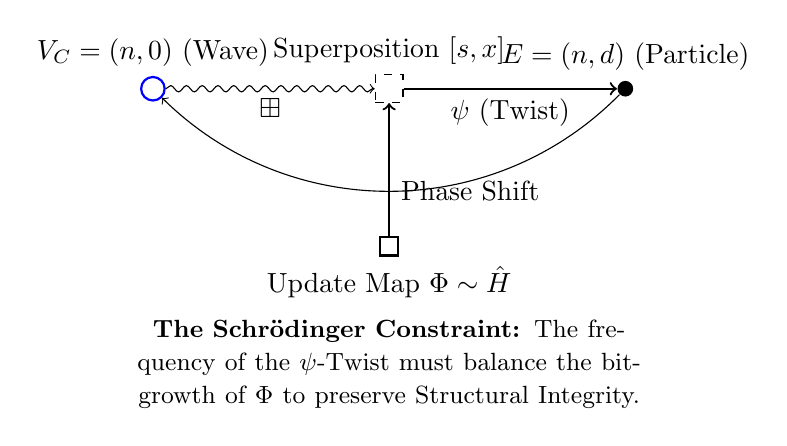
\begin{tikzpicture}[node distance=2cm, auto]
    % Wave to Particle Resolution Visualization
    \node (wave) at (0,2) [circle, draw, blue, thick, inner sep=3pt, label=above:{$V_C = (n, 0)$ (Wave)}] {};
    \node (susp) at (3,2) [rectangle, draw, dashed, inner sep=5pt, label=above:{Superposition $[s, x]$}] {};
    \node (part) at (6,2) [circle, fill, black, inner sep=2pt, label=above:{$E = (n, d)$ (Particle)}] {};
    
    \node (phi) at (3,0) [rectangle, draw, thick, label=below:{Update Map $\Phi \sim \hat{H}$}] {};

    \draw [->, decorate, decoration={snake, amplitude=.4mm, segment length=2mm}] (wave) -- (susp) node [midway, below] {$\boxplus$};
    \draw [->, thick] (susp) -- (part) node [midway, below] {$\psi$ (Twist)};
    
    \draw [->, bend left=45] (part) to node [right] {Phase Shift} (wave);
    \draw [->, thick] (phi) -- (susp);
    
    \node at (3,-1.5) [text width=8cm, align=center] {\small \textbf{The Schrödinger Constraint:} The frequency of the $\psi$-Twist must balance the bit-growth of $\Phi$ to preserve Structural Integrity.};
\end{tikzpicture}
\caption{Visualization of the Discrete Schrödinger Resolution. The transition from wave-like vacuum to localized particle is mediated by the $\psi$ operator, whose latency determines the emergent time evolution of the system.}
\end{figure}

\end{document}